\documentclass{article}
\usepackage{amsmath}
\usepackage{amsfonts}
\usepackage{amssymb}
\usepackage{cancel}

\usepackage{graphicx}


\setlength\parindent{0pt}

\author{Pranav Tikkawar}
\title{Homework 4: 292H}

\begin{document}
\maketitle
\section*{Question 1}
Compute $e^{tA}$ for the matrix $$A = \begin{bmatrix}
    -1 & 2 & 2 \\
    -2 & -1 & 1 \\
    -2 & -1 & -1
\end{bmatrix}$$ 
The eigenvalues of the matrix is given by $A - \mu I = \begin{bmatrix}
    -1 - \mu & 2 & 2 \\
    -2 & -1 - \mu & 1 \\
    -2 & -1 & -1 - \mu
\end{bmatrix} $
The charecteristic polynomial of the matrix is given by
$$(-1 - \mu)[(-1-\mu)(-1-\mu) + 1] - 2[2(-1-\mu) - 2] + 2[2(-1-\mu) + 2] $$
$$-\mu^3 - 3 \mu^2 - 12\mu - 10 $$
$$(-\mu -1)(\mu^2 + 2\mu + 10)$$
The roots of the charecteristic polynomial are $\mu_1 = -1, \mu_2 = -1-3i, \mu_3 = -1+3i$.\\
The eigenvector for the eigenvalue $\mu_1 = -1$ is given by solving the equation $(A + I)X = 0$. Here the matrix $[A + I | 0]$ is given by
$$\begin{bmatrix}
    0 & 2 & 2 & 0\\
    -2 & 0 & 1 & 0\\
    -2 & -1 & 0 &0
\end{bmatrix} $$
The reduced row echelon form of the matrix is
$$ \begin{bmatrix}
    -2 & 0 & 1 & 0\\
    0 & -1 & -1 & 0\\
    0 & 2 & 2 & 0
\end{bmatrix}, 
\begin{bmatrix}
    2 & 0 & -1 & 0\\
    0 & 1 & 1 & 0\\
    0 & 0 & 0 & 0
\end{bmatrix}$$
Thus the eigenvector for the eigenvalue $\mu_1 = -1$ is given by
$$\begin{bmatrix}
    1\\
    -2\\
    2
\end{bmatrix} $$
The eigenvector for the eigenvalue $\mu_2 = -1-3i$ is given by solving the equation $(A - (-1-3i) I)X = 0$. Here the matrix $[A - (-1-3i) I | 0]$ is given by
$$\begin{bmatrix}
    3i & 2 & 2 & 0\\
    -2 & 3i & 1 & 0\\
    -2 & -1 & 3i & 0
\end{bmatrix} $$
The reduced row echelon form of the matrix is
$$ \begin{bmatrix}
    3i & 2 & 2 & 0\\
    0 & 5i/3 & 1-4i/3 & 0\\
    0 & -1-4i/3 & 5i/3 & 0
\end{bmatrix} \begin{bmatrix}
    3i & 2 & 2 & 0\\
    0 & 5i/3 & 1-4i/3 & 0\\
    0 & 0 & 0 & 0
\end{bmatrix}\begin{bmatrix}
    3i & 2 & 2 & 0\\
    0 & 1 & -4/5 - 3i/5 & 0\\
    0 & 0 & 0 & 0
\end{bmatrix} $$ $$ \begin{bmatrix}
    3i & 0 & 18/5 + 6i/5 & 0\\
    0 & 1 & -4/5 - 3i/5 & 0\\
    0 & 0 & 0 & 0
\end{bmatrix} \begin{bmatrix}
    1 & 0 & 2/5 - 6i/5 & 0\\
    0 & 1 & -4/5 - 3i/5 & 0\\
    0 & 0 & 0 & 0
\end{bmatrix}$$
This leads us to a system of equations 
$$\begin{cases}
    5x + (2 - 6i)z = 0\\
    5y - (4 + 3i)z = 0
\end{cases}$$
Thus the eigenvector for the eigenvalue $\mu_2 = -1-3i$ is given by
$$\begin{bmatrix}
    -2 + 6i\\
    4 + 3i\\
    5
\end{bmatrix} $$
We can get 2 linearly indpendent general solutions from the real and imaginary parts. 
$$ e^{tA} = e^{-t} (cos(-3t) + isin(-3t)) \begin{bmatrix}
    -2 + 6i\\
    4 + 3i\\
    5
\end{bmatrix}$$
$$ e^{-t}\begin{bmatrix}
    2cos(3t) - 6sin(3t)\\
    4cos(3t) - 3sin(3t)\\
    5cos(3t)
\end{bmatrix} + e^{-t}\begin{bmatrix}
    6cos(3t) - 2sin(3t) \\
    3cos(3t) + 4sin(3t)\\
    5sin(3t)
\end{bmatrix} $$
When we make $e^{tA}$, we can use the real and imaginary solution as different linearly indpendent solutions. Thus the solution to the system of differential equations is given by
$$e^{tA} = e^{-t}\begin{bmatrix}
    1\\
    -2\\
    2
\end{bmatrix} + e^{-t}\begin{bmatrix}
    2cos(3t) - 6sin(3t)\\
    4cos(3t) - 3sin(3t)\\
    5cos(3t)
\end{bmatrix} + e^{-t}\begin{bmatrix}
    6cos(3t) - 2sin(3t) \\
    3cos(3t) + 4sin(3t)\\
    5sin(3t)
\end{bmatrix}$$
\subsection*{a}
Yes it does converge to zero. It does so at a rate of $e^{-t}$ as it is the term with most "power". 
\subsection*{b}
The intial points that would lead to a spiral would be any intial points that are in the form $$ \begin{bmatrix}
    0 \\
    a\\
    b\\
\end{bmatrix}
$$ for $a,b \in \mathbb{R}$ and $a,b\neq 0$. \
\subsection*{c}
It would be $\frac{2 \pi}{3} $ as the period of the solution since there is a $t3$ in the argument of the cosine and sine functions.
\section*{Question 2}
$$A = \begin{bmatrix}
    -4 & 2 & 7\\
    -1 & -1 & -1\\
    -1 & 2 & 4
\end{bmatrix}$$
The eigenvalues of the matrix are 
$$\mu = 1, 1, -3 $$
The eigenvector for the eigenvalue $1$ is 
$$ \begin{bmatrix}
    1\\
    -1\\
    1
\end{bmatrix}$$
The eigenvector for the eigenvalue $-3$ is
$$ \begin{bmatrix}
    2\\
    1\\
    0
\end{bmatrix}$$
To get get $e^{tA}$ we need to use the JC form of the matrix. 
$$ P =  \begin{bmatrix}
    1 & ? & 2\\
    -1 & ? & 1\\
    1 & ? & 0
\end{bmatrix}, U = \begin{bmatrix}
    1 & 1 & 0\\
    0 & 1 & 0\\
    0 & 0 & -3
\end{bmatrix} $$
To find the 2nd column of $P$, we can find $(A - 1I)w = v$ where $v$ is the eigenvector for the eigenvalue $1$ and $w$ is the generalized eigenvector. Thus we need a augmented matrix $[A - I | v]$.
$$\begin{bmatrix}
    -5 & 2 & 7 & 1\\
    -1 & -2 & -1 & -1\\
    -1 & 2 & 3 & 1
\end{bmatrix}$$
The reduced row echelon form of the matrix is
$$\begin{bmatrix}
    1 & 0 & -1 & 0\\
    0 & 1 & 1 & 1/2\\
    0 & 0 & 0 & 0
\end{bmatrix}$$
Thus the generalized eigenvector is given by the system
$$\begin{cases}
    x - z = 0\\
    y + z = 1/2
\end{cases}$$
Thus the generalized eigenvector is given by
$$\begin{bmatrix}
    0\\
    1/2\\
    0
\end{bmatrix}$$
Thus the matrix $P$ is given by
$$\begin{bmatrix}
    1 & 0 & 2\\
    -1 & 1/2 & 1\\
    1 & 0 & 0
\end{bmatrix}$$
Thus the matrix $P^{-1}$ is given by
$$\begin{bmatrix}
    0 & 0 & 1\\
    -1 & 2 & 3\\
    0.5 & 0 & -0.5
\end{bmatrix}$$
The matrix $e^{tU}$ is given by $e^{tD}e^{tN}$
$$\begin{bmatrix}
    e^t & 0 & 0\\
    0 & e^t & 0\\
    0 & 0 & e^{-3t}
\end{bmatrix}(tN + I)$$
$$\begin{bmatrix}
    e^t & 0 & 0\\
    0 & e^t & 0\\
    0 & 0 & e^{-3t}
\end{bmatrix} \begin{bmatrix}
        1 & t & 0\\
        0 & 1 & 0\\
        0 & 0 & 1
    \end{bmatrix}$$
$$\begin{bmatrix}
        e^t & te^t & 0\\
        0 & e^t & 0\\
        0 & 0 & e^{-3t}
\end{bmatrix}$$
Thus the matrix $e^{tA}$ is given by
$$P e^{tU} P^{-1}$$
$$\begin{bmatrix}
    1 & 0 & 2\\
    -1 & 1/2 & 1\\
    1 & 0 & 0
\end{bmatrix} \begin{bmatrix}
    e^t & te^{t} & 0\\
    0 & e^t & 0\\
    0 & 0 & e^{-3t}
\end{bmatrix} \begin{bmatrix}
    0 & 0 & 1\\
    -1 & 2 & 3\\
    0.5 & 0 & -0.5
\end{bmatrix}$$
\section*{Question 3}
Phase Portrait of the system of differential equations: $v_1 = \begin{bmatrix}
    -1 \\
    0
\end{bmatrix}, v_2 = \begin{bmatrix}
    2  \\
    1
\end{bmatrix}$
\subsection*{a}
$A$ has -2, -1 as eigenvalues. \\
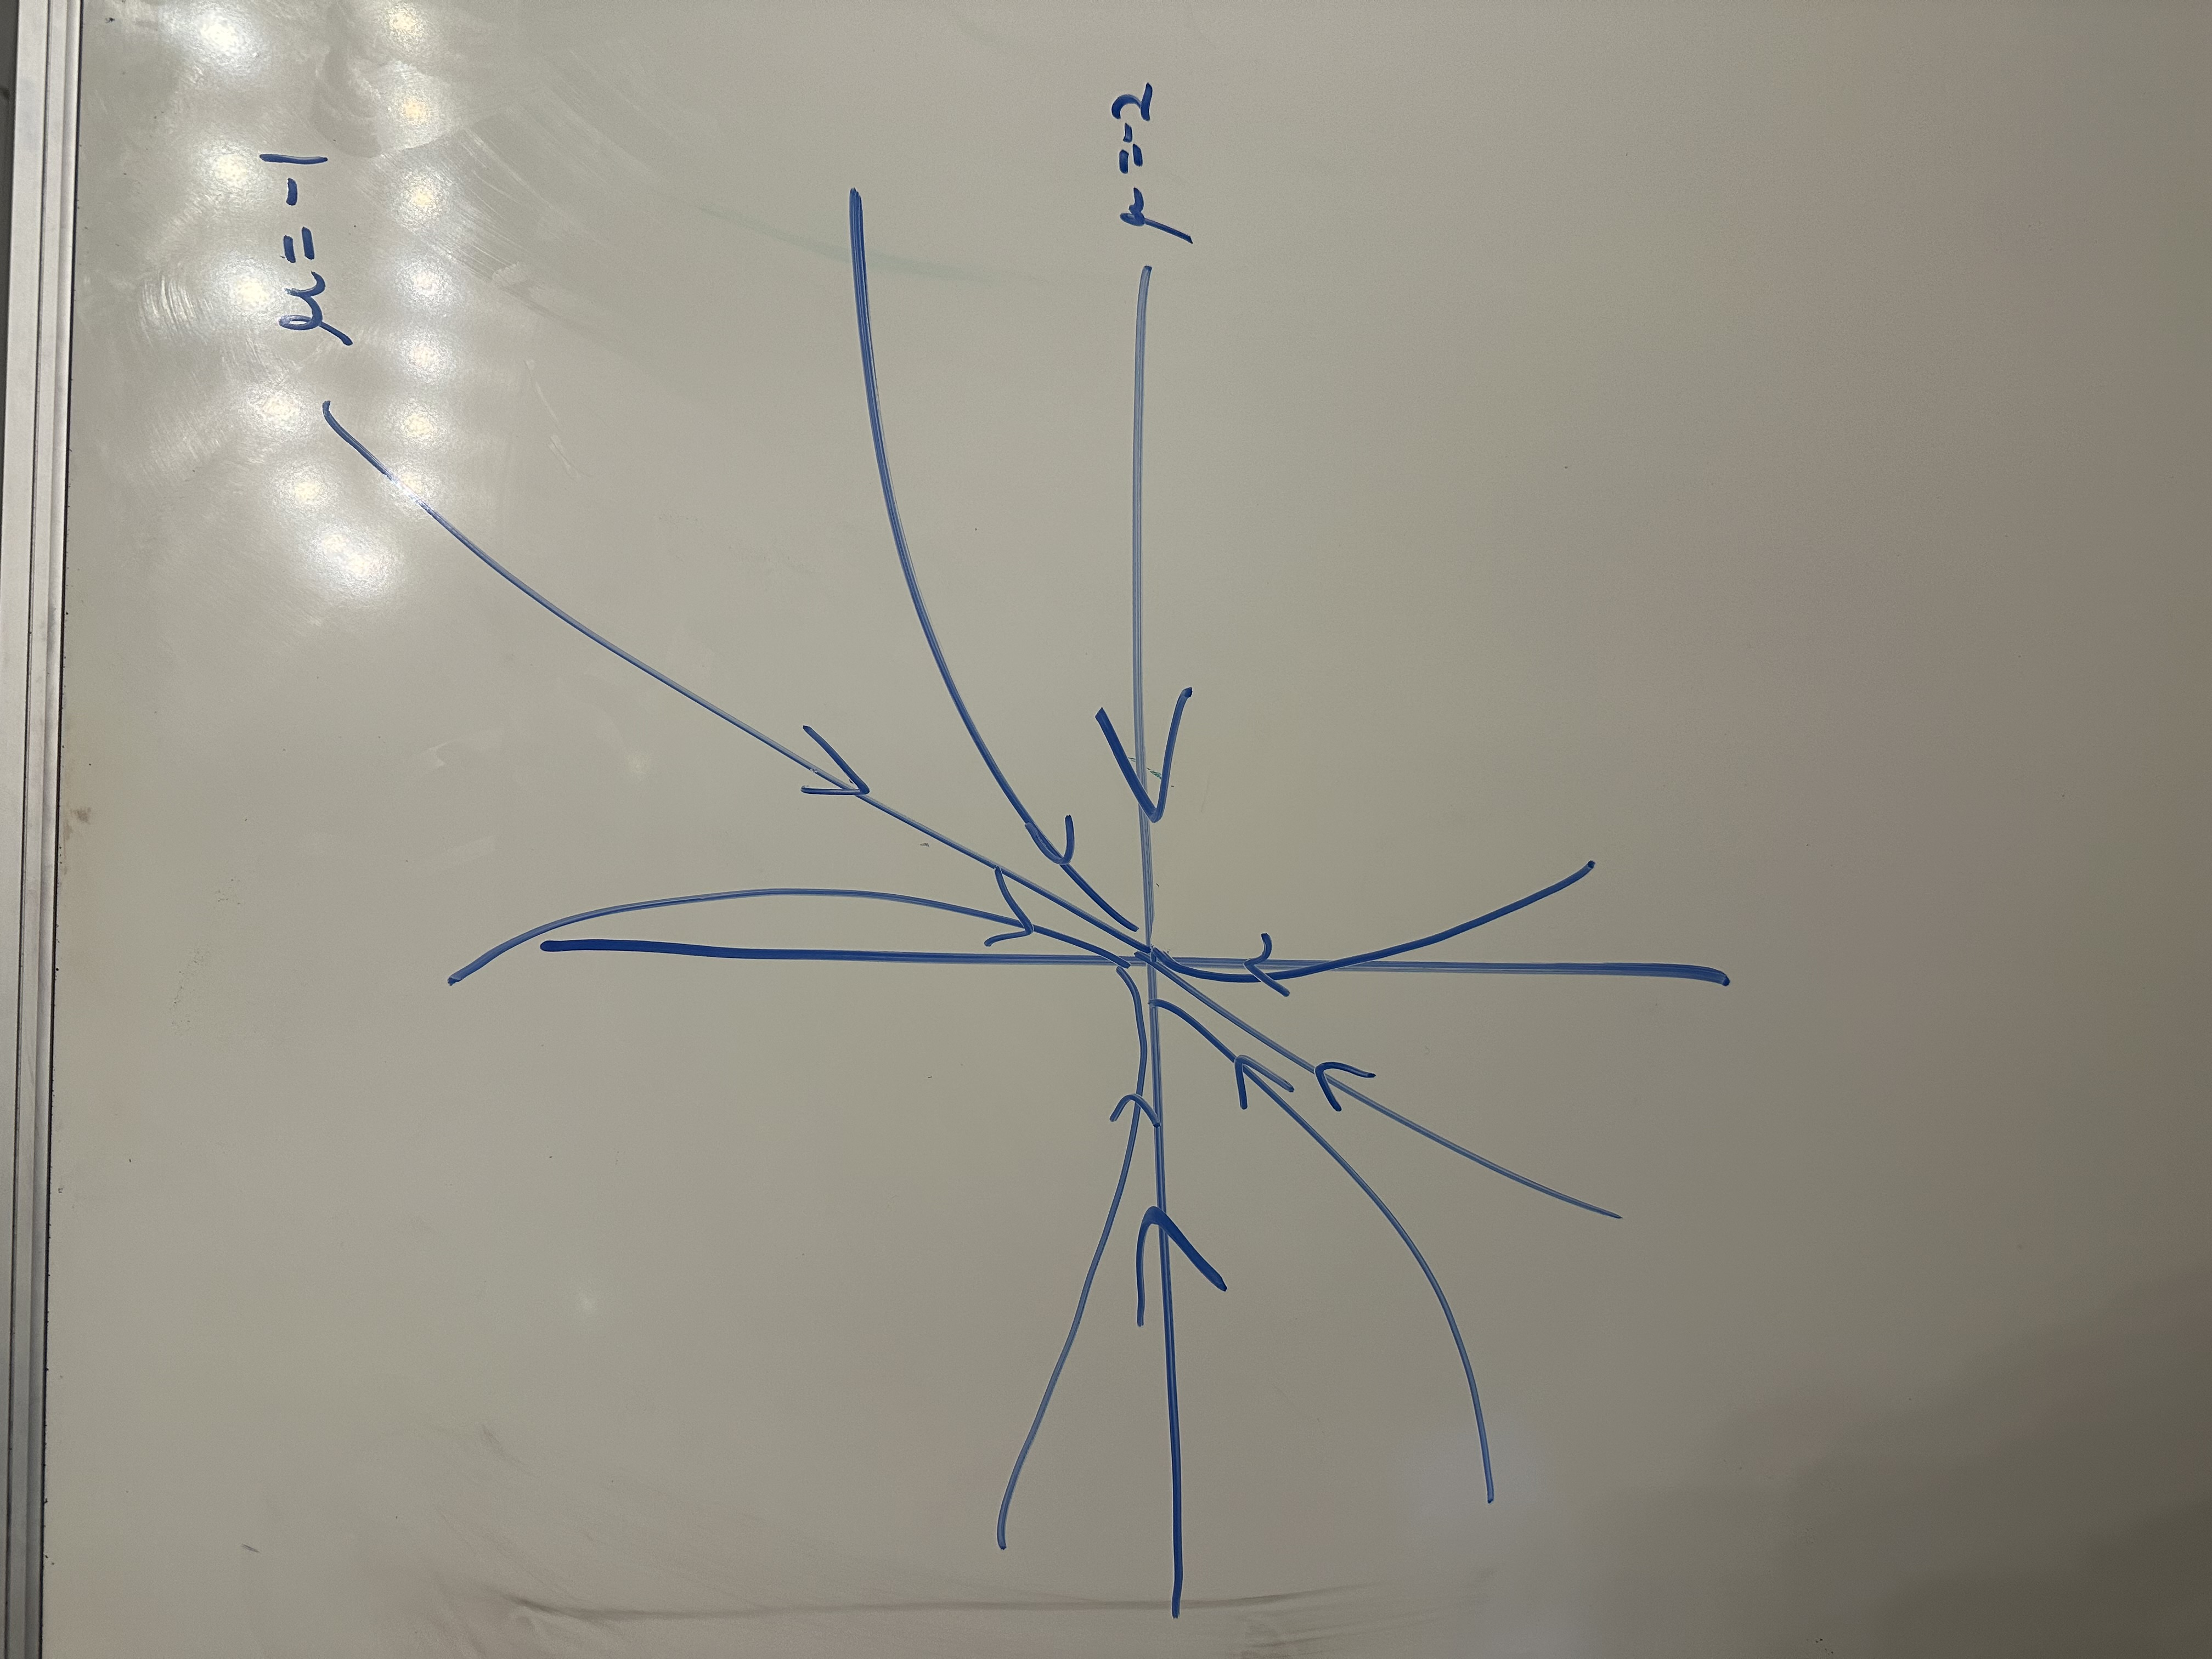
\includegraphics[width=0.5\textwidth]{IMG_2796.jpg}
\subsection*{b}
$A$ has -2, 1 as eigenvalues. \\
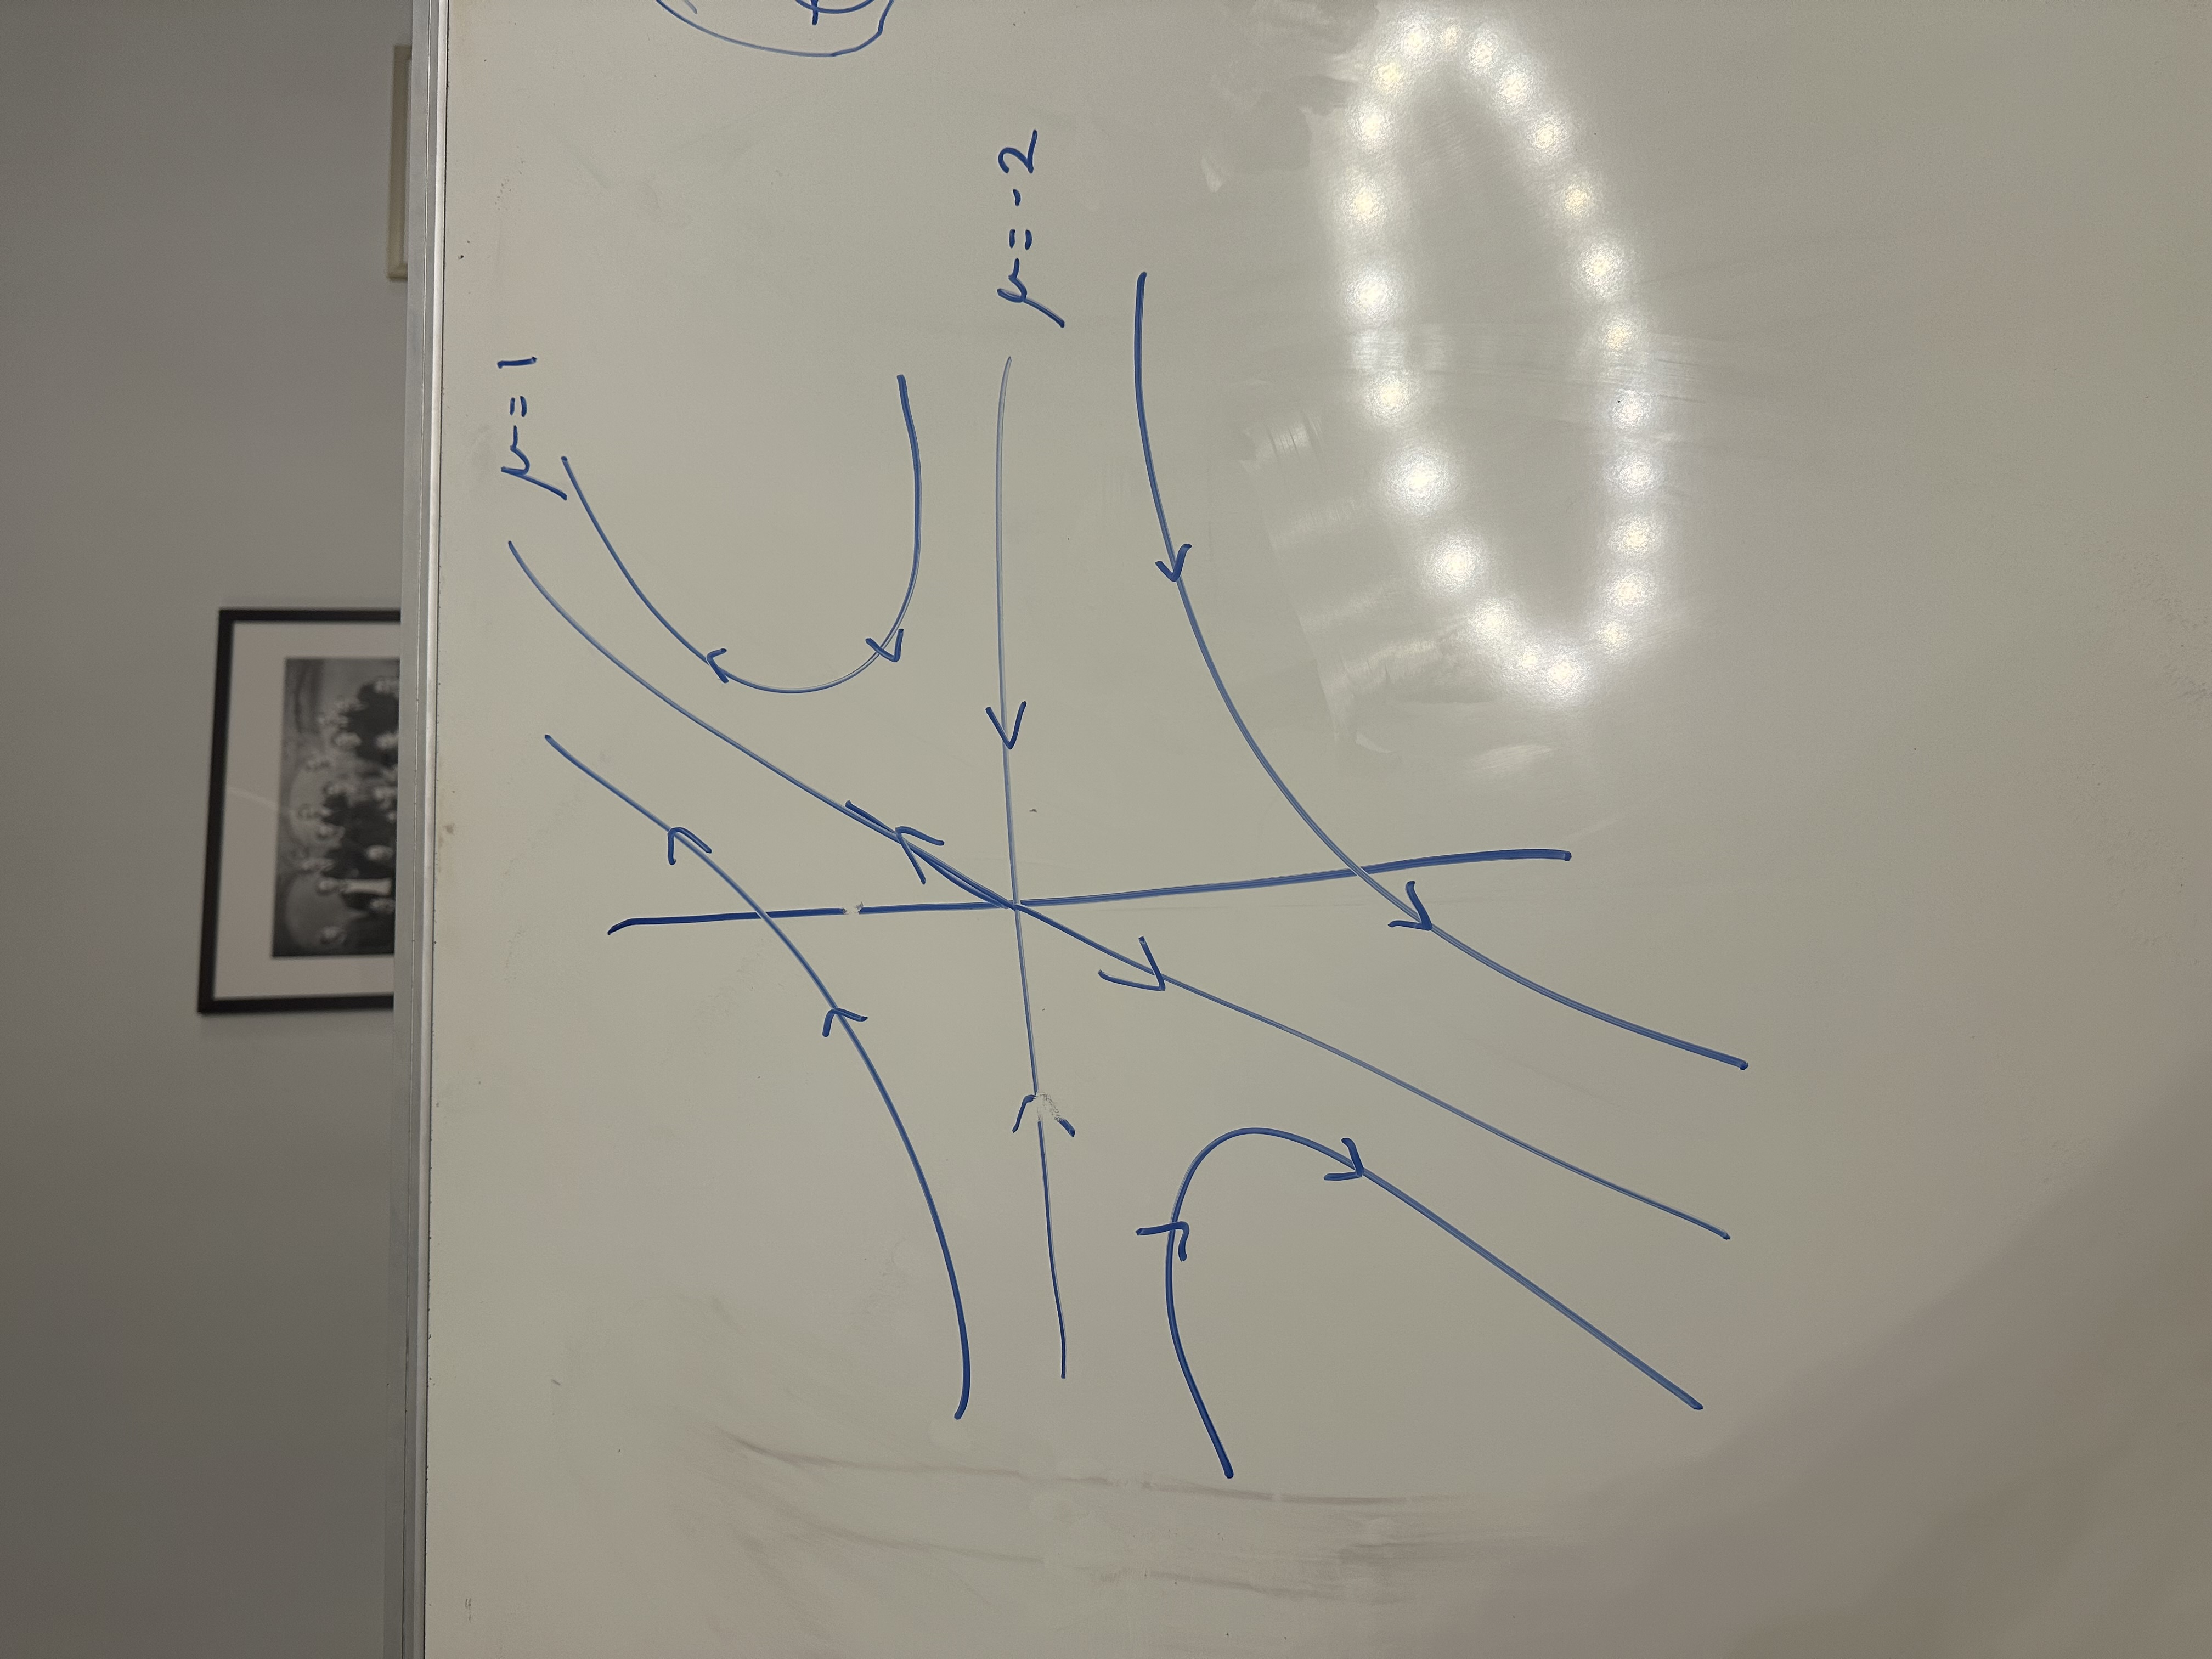
\includegraphics[width=0.5\textwidth]{IMG_2797.jpg}
\subsection*{c}
$A$ has 2, 1 as eigenvalues.\\
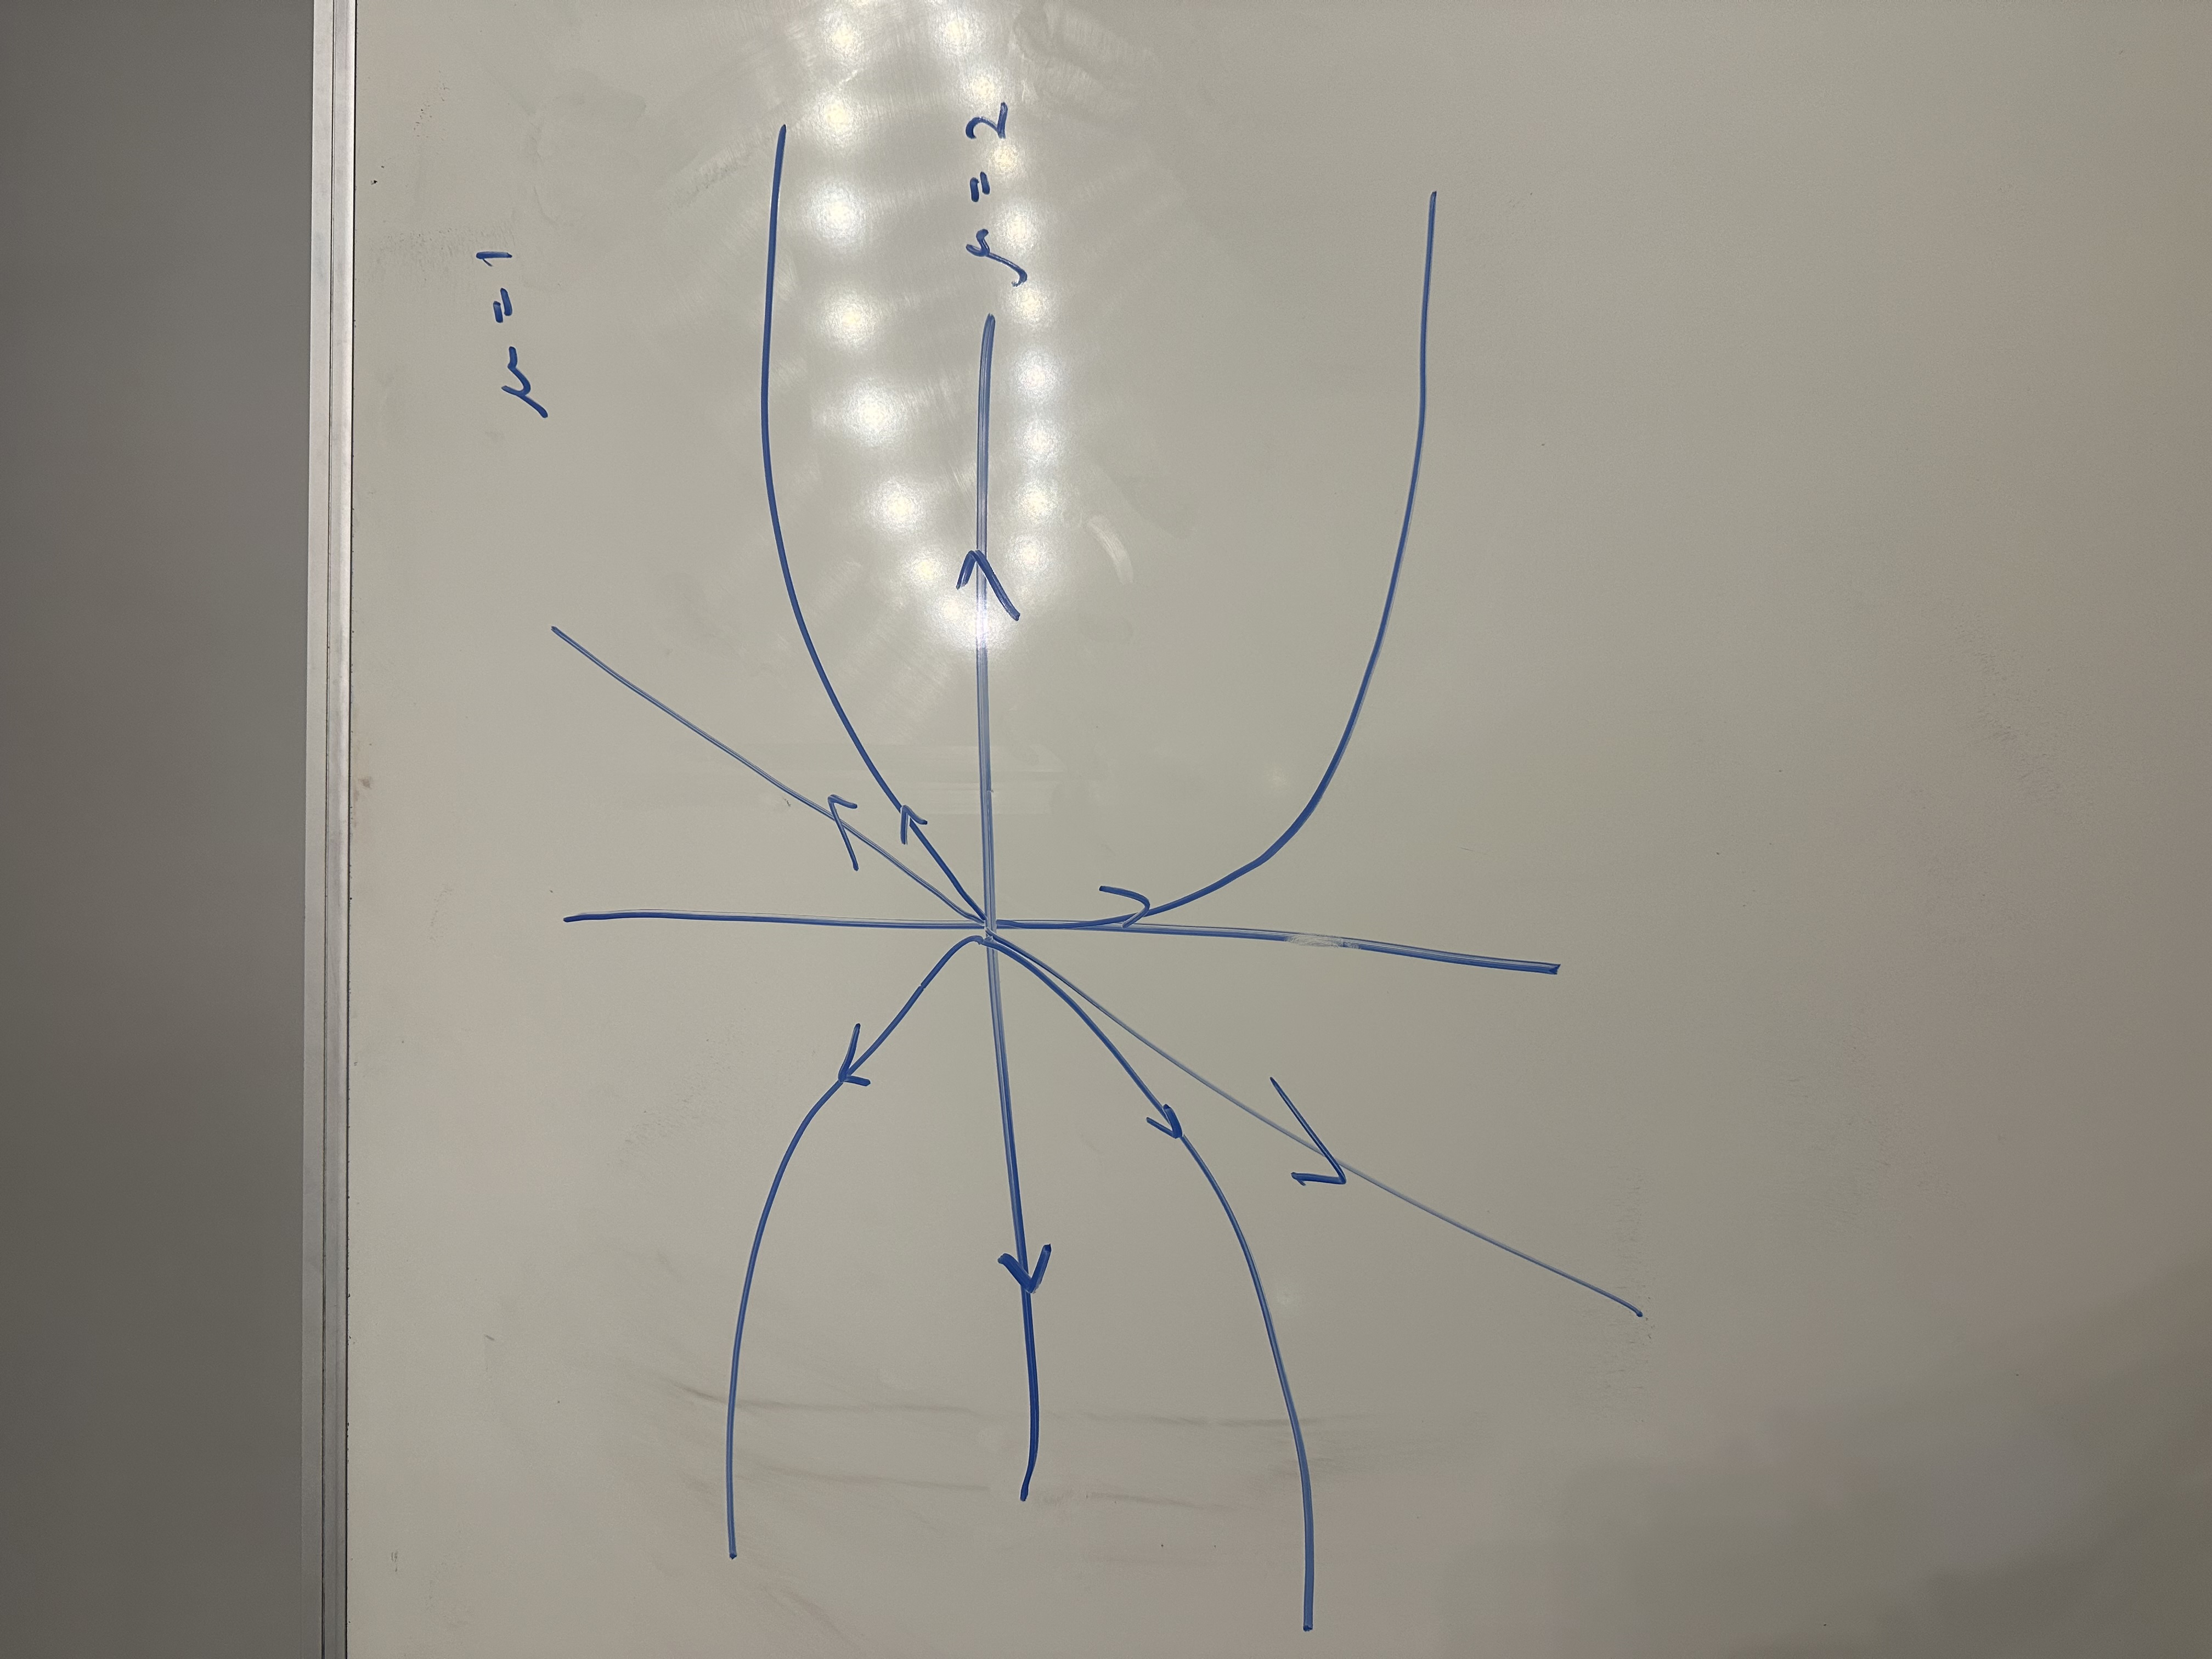
\includegraphics[width=0.5\textwidth]{IMG_2798.jpg}
\subsection*{d}
$A$ has -2, 0 as eigenvalues.\\
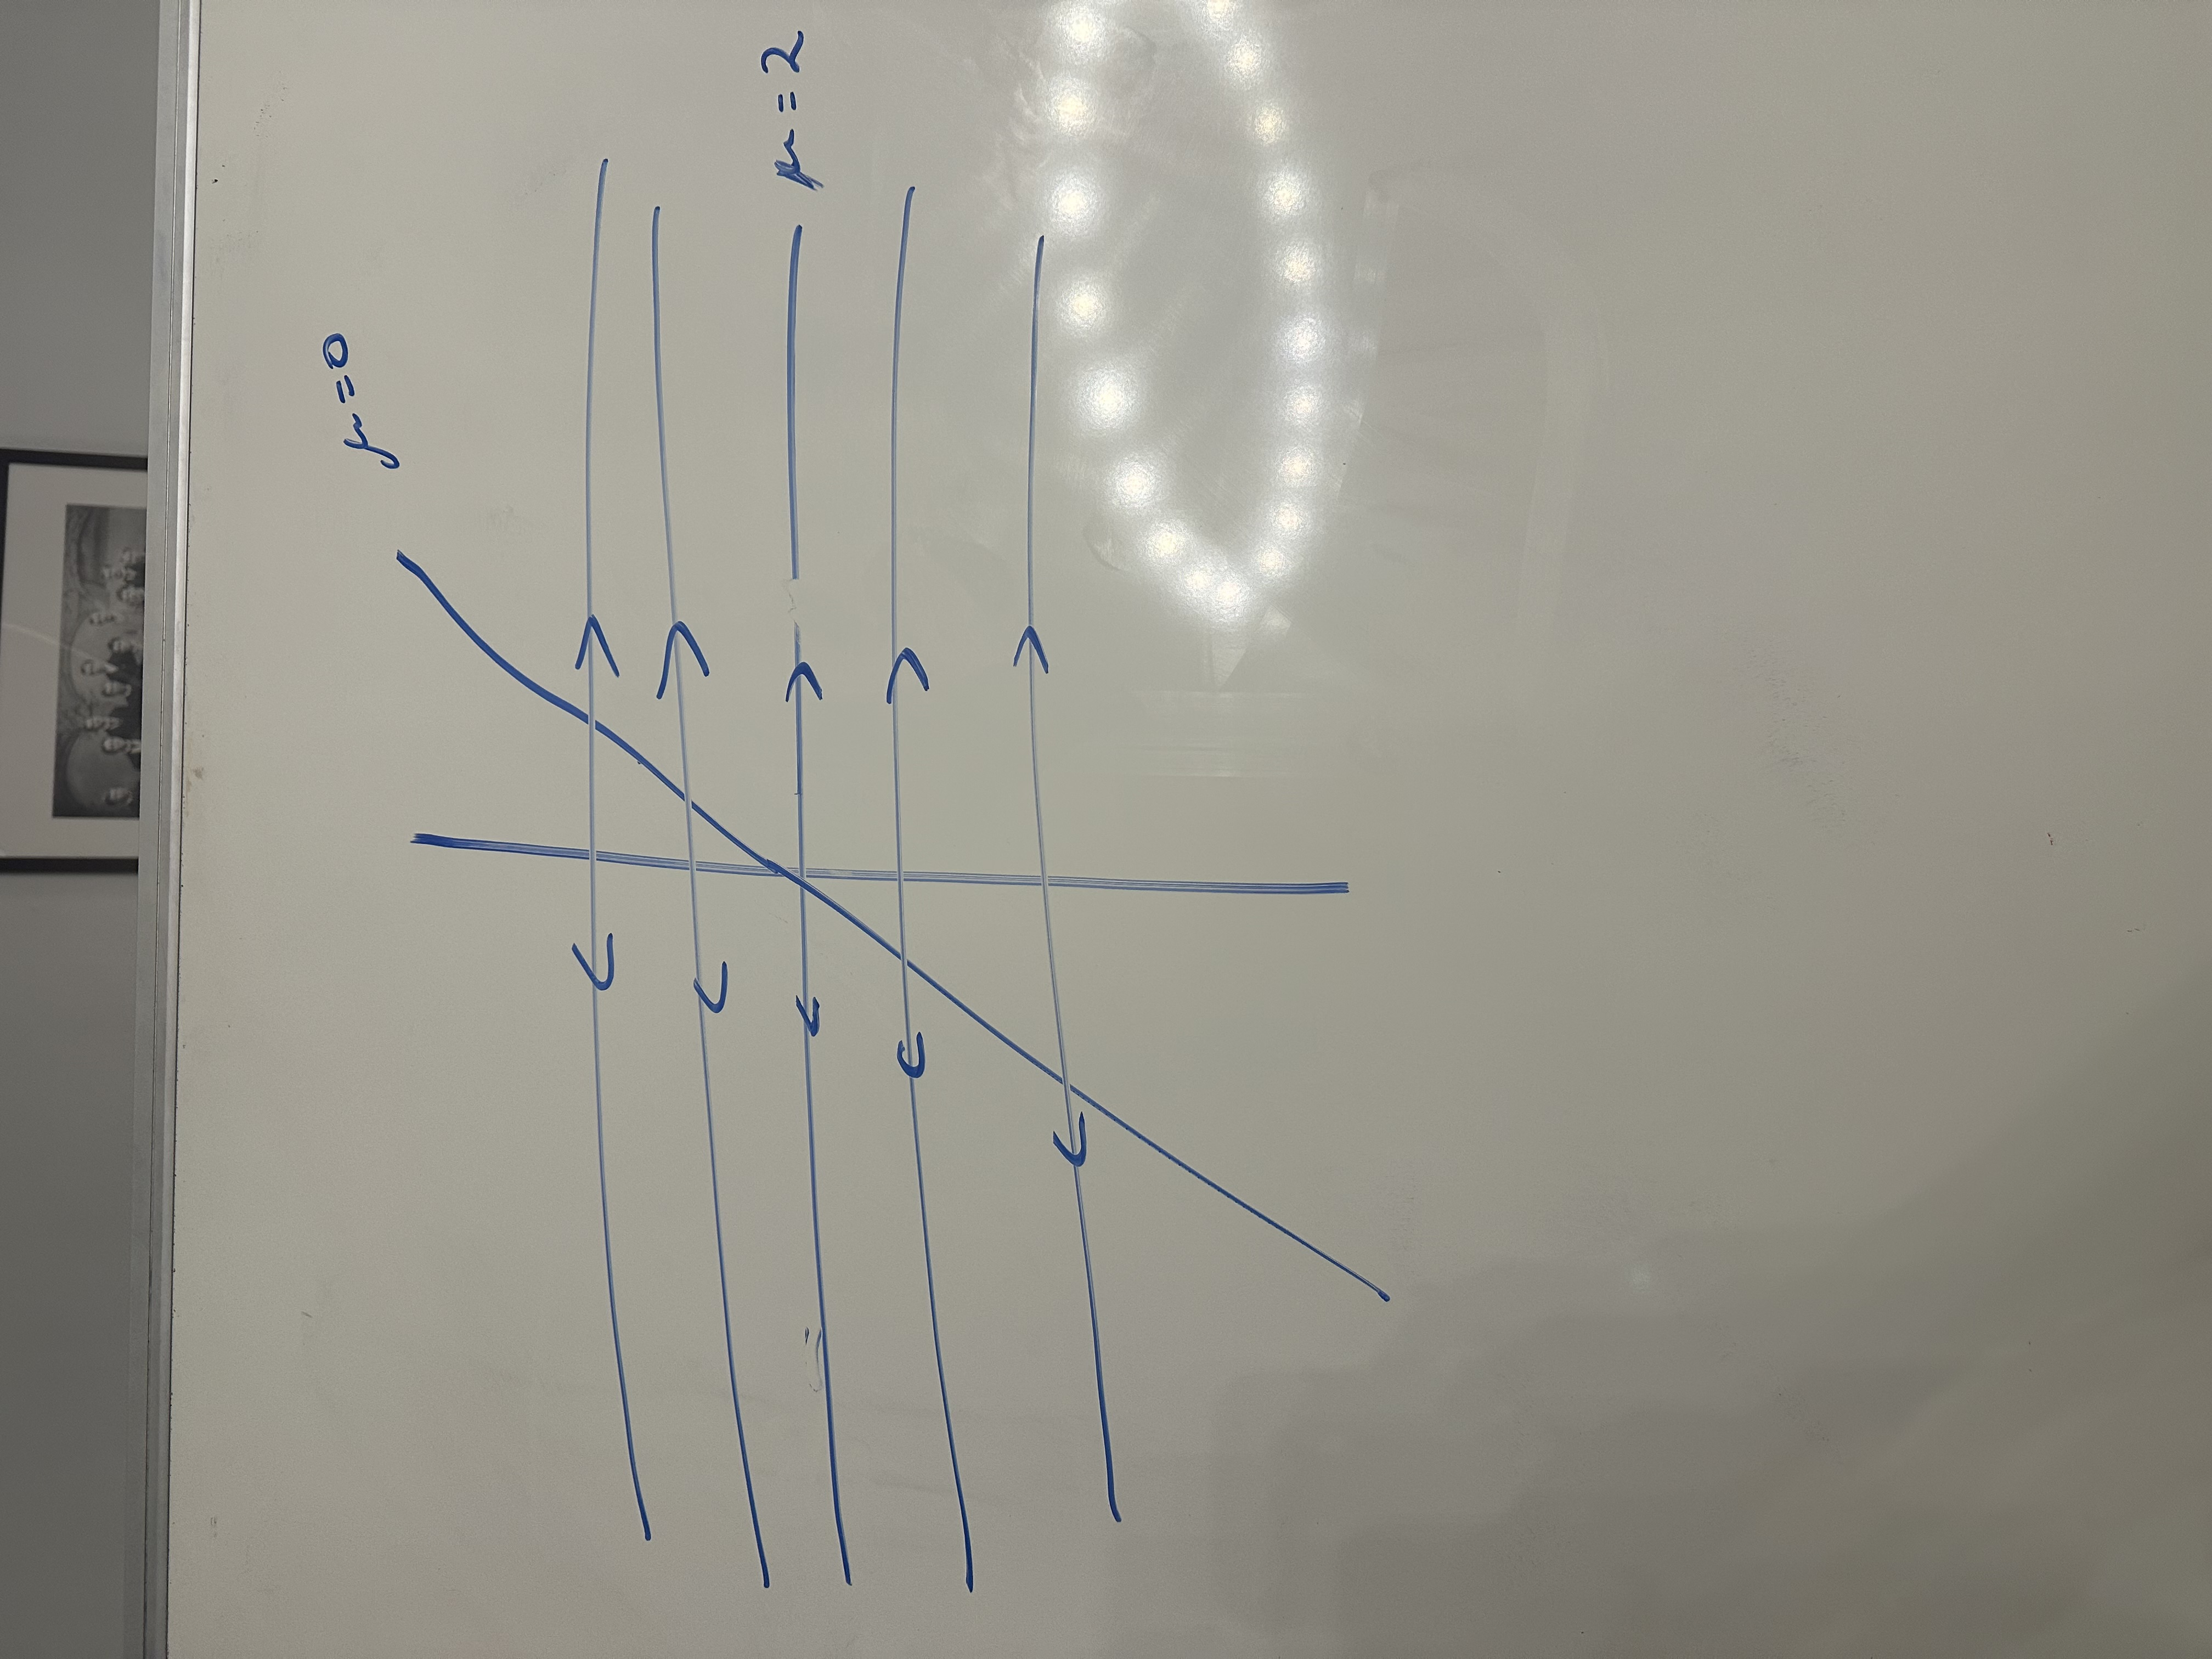
\includegraphics[width=0.5\textwidth]{IMG_2799.jpg}
\subsection*{e}
$A$ has 2 as repeaded eigenvalues with 2 LI eigenvectors.\\
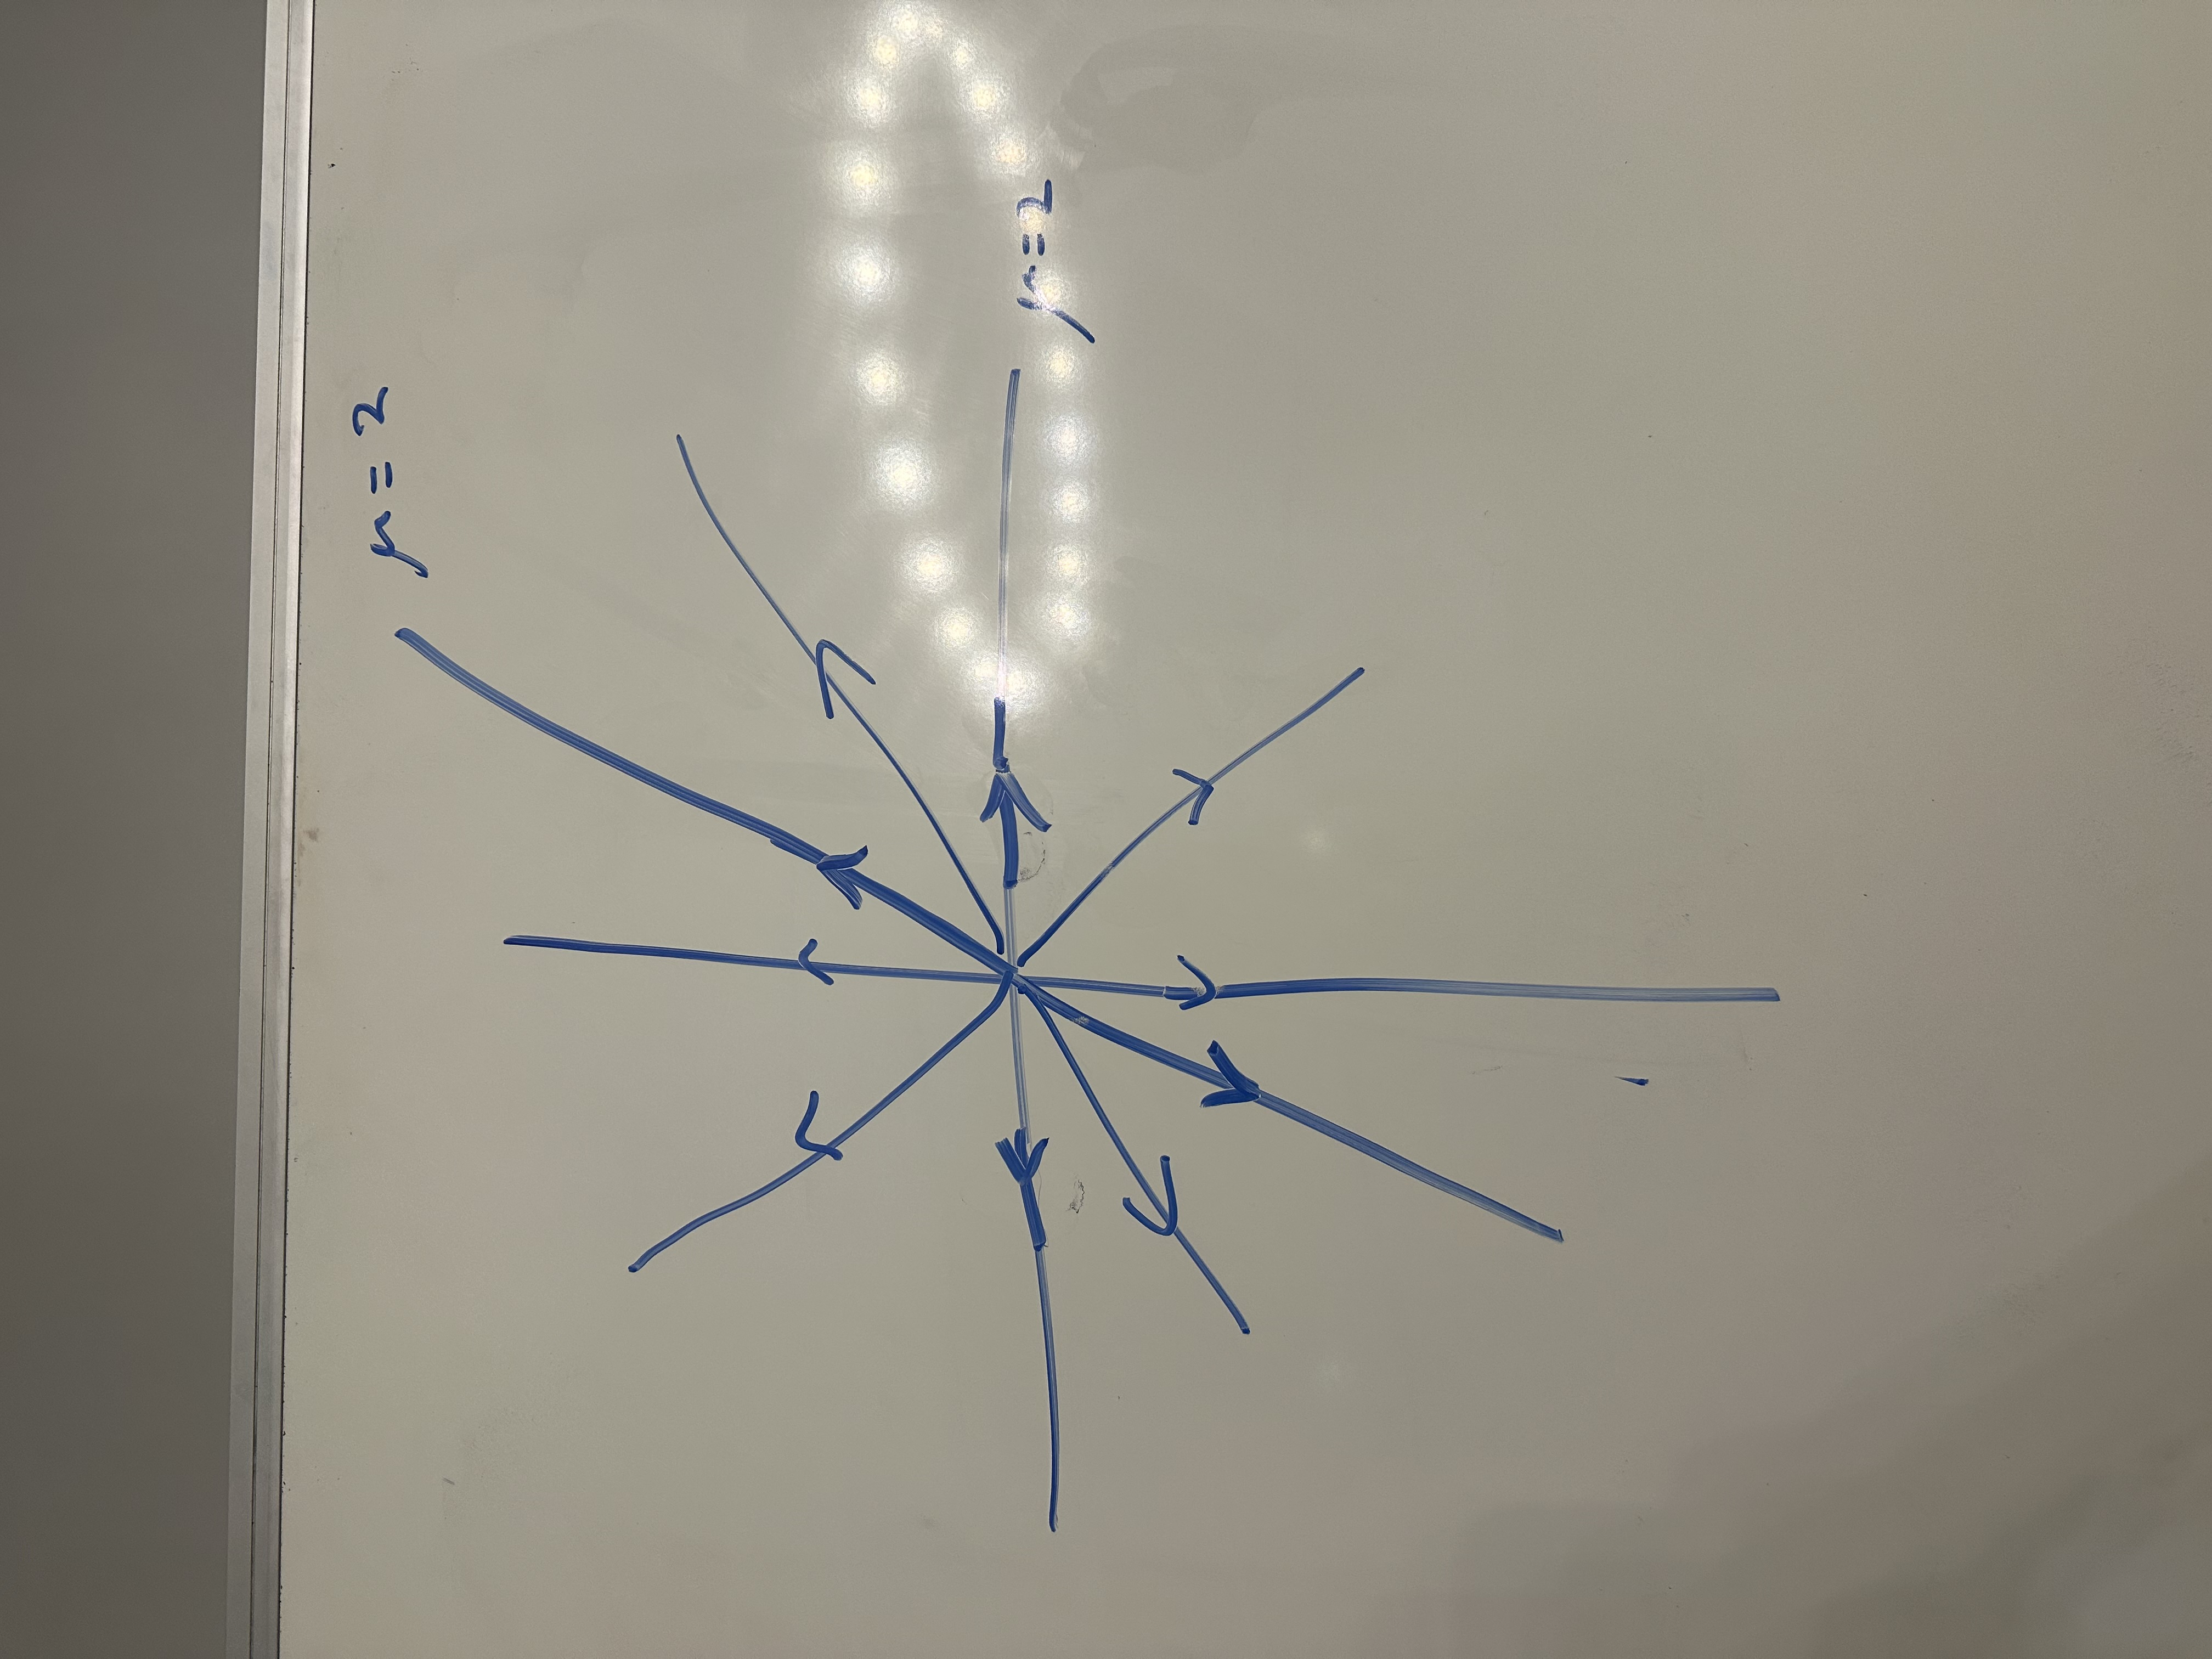
\includegraphics[width=0.5\textwidth]{IMG_2800.jpg}
\subsection*{f}
$A$ has 2 as repeated eigenvalues with 1 LI eigenvector.\\
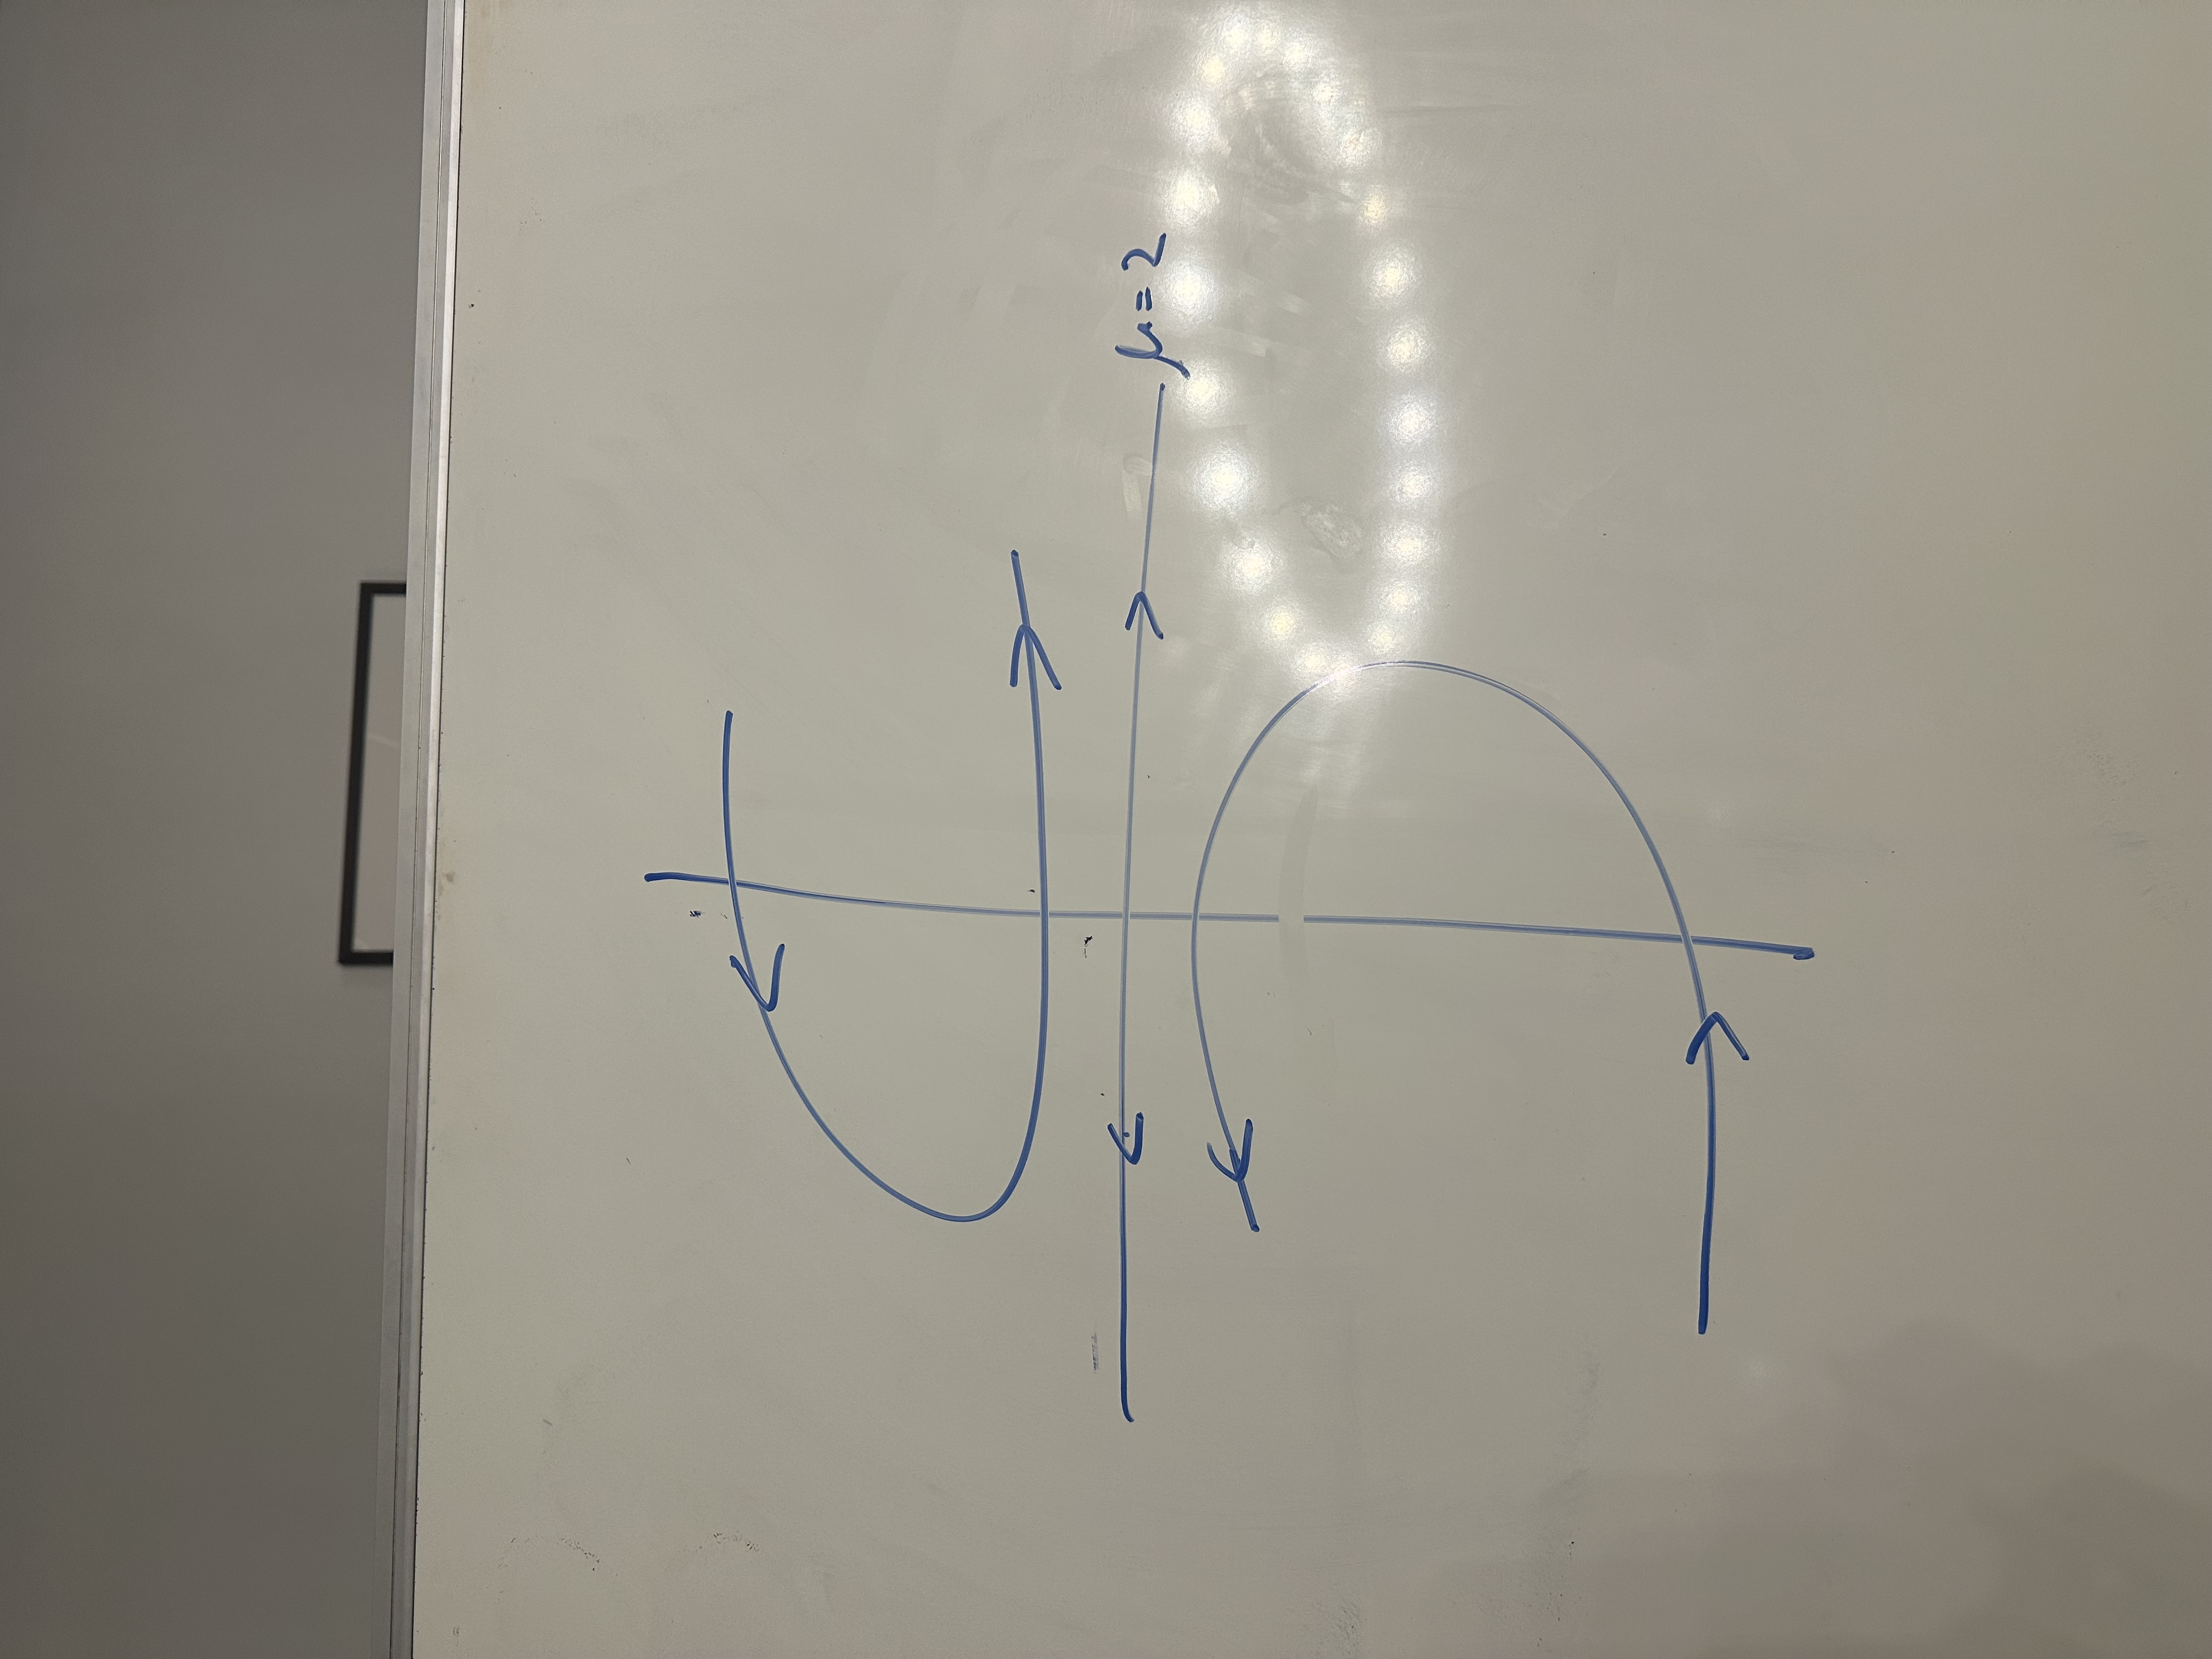
\includegraphics[width=0.5\textwidth]{IMG_2801.jpg}

\section*{Question 4}
Solve $X'(t) = \begin{bmatrix}
    0 & -1\\
    -2 & 1
\end{bmatrix}X(t) + \begin{bmatrix}
    te^{-2t}  \\
    e^{-2t}
\end{bmatrix}$
With initial condition $X(0) = X_0$
Using Duhamels formula we can see the solution will be in the form of 
$$X(t) = e^{(t-t_0)A}X(0) + \int_{t_0}^t e^{(t-s)A}g(s)ds$$ 
To get $e^{(t-t_0)A}$ we need to find the eigenvalues of the matrix $A = \begin{bmatrix}
    0 & -1\\
    -2 & 1
\end{bmatrix}$. The charecteristic polynomial of the matrix is given by
$$\begin{vmatrix}
    -\lambda & -1\\
    -2 & 1 - \lambda
\end{vmatrix} = \lambda^2 - \lambda - 2 = 0$$
Thus the eigenvalues of the matrix are $\mu_1 = -1, \mu_2 = 2$. 
The eigenvector for the eigenvalue $\mu_1 = -1$ is given by solving the equation $(A + I)X = 0$. Here the matrix $[A + I | 0]$ is given by
$$\begin{bmatrix}
    1 & -1\\
    -2 & 2
\end{bmatrix} $$
The reduced row echelon form of the matrix is
$$ \begin{bmatrix}
    1 & -1\\
    0 & 0
\end{bmatrix}$$
Thus the eigenvector for the eigenvalue $\mu_1 = -1$ is given by
$$\begin{bmatrix}
    1\\
    1
\end{bmatrix} $$
The eigenvector for the eigenvalue $\mu_2 = 2$ is given by solving the equation $(A - 2I)X = 0$. Here the matrix $[A - 2I | 0]$ is given by
$$\begin{bmatrix}
    -2 & -1\\
    -2 & -1
\end{bmatrix} $$
The reduced row echelon form of the matrix is
$$ \begin{bmatrix}
    1 & 1/2\\
    0 & 0
\end{bmatrix}$$
Thus the eigenvector for the eigenvalue $\mu_2 = 2$ is given by
$$\begin{bmatrix}
    -1\\
    2
\end{bmatrix} $$
Thus the matrix $e^{(t-t_0)A}$ is given by
$$ \begin{bmatrix}
    1 & -1\\
    1 & 2
\end{bmatrix} \begin{bmatrix}
    e^{-(t-t_0)} & 0\\
    0 & e^{2(t-t_0)}
\end{bmatrix} \begin{bmatrix}
    2/3 & 1/3\\
    -1/3 & 1/3
\end{bmatrix}$$
$$\begin{bmatrix}
    e^{t_0-t} & -e^{2(t-t_0)}\\
    e^{t_0-t} & 2e^{2(t-t_0)}
\end{bmatrix} \begin{bmatrix}
    2/3 & 1/3\\
    -1/3 & 1/3
\end{bmatrix} $$
$$\begin{bmatrix}
    \frac{2e^{-(t-t_0)}}{3} + \frac{e^{2(t-t_0)}}{3} & \frac{e^{-(t-t_0)}}{3} - \frac{e^{2(t-t_0)}}{3}\\
    \frac{2e^{-(t-t_0)}}{3} - \frac{2e^{2(t-t_0)}}{3} & \frac{e^{-(t-t_0)}}{3} + \frac{2e^{2(t-t_0)}}{3}
\end{bmatrix}
$$
Now we need to find the integral of $e^{(t-s)A}g(s)ds$. 
$$\int_{0}^{t}\begin{bmatrix}
    \frac{2e^{-(t-s)}}{3} + \frac{e^{2(t-s)}}{3} & \frac{e^{-(t-s)}}{3} - \frac{e^{2(t-s)}}{3}\\
    \frac{2e^{-(t-s)}}{3} - \frac{2e^{2(t-s)}}{3} & \frac{e^{-(t-s)}}{3} + \frac{2e^{2(t-s)}}{3}
\end{bmatrix} \begin{bmatrix}
    se^{-2s}  \\
    e^{-2s}
\end{bmatrix}ds $$
The multiplication is:
$$\frac{1}{3}\int_{0}^{t}\begin{bmatrix}
    se^{-2s}(\frac{2e^{-(t-s)}}{3} + \frac{e^{2(t-s)}}{3}) + e^{-2s}(\frac{2e^{-(t-s)}}{3} - \frac{2e^{2(t-s)}}{3}) \\
    se^{-2s}(\frac{e^{-(t-s)}}{3} - \frac{e^{2(t-s)}}{3}) + e^{-2s}(\frac{e^{-(t-s)}}{3} + \frac{2e^{2(t-s)}}{3})
\end{bmatrix} ds$$
We can split this integral into its components. The first component integrates to:
$$ -\frac{1}{144}  e^{-2t}[7e^{4t}-64e^{t}+36t+57]$$

The second component integrates to:
$$ \frac{1}{144}  e^{-2t}[7e^{4t}-32e^{t}+12t-39]$$
Thus our final solution is given by
$$X(t) = \begin{bmatrix}
    \frac{2e^{-(t)}}{3} + \frac{e^{2(t)}}{3} & \frac{e^{-(t)}}{3} - \frac{e^{2(t)}}{3}\\
    \frac{2e^{-(t)}}{3} - \frac{2e^{2(t)}}{3} & \frac{e^{-(t)}}{3} + \frac{2e^{2(t)}}{3}
\end{bmatrix}  X_0 + \begin{bmatrix}
    -\frac{1}{144}  e^{-2t}[7e^{4t}-64e^{t}+36t+57] \\
    \frac{1}{144}  e^{-2t}[7e^{4t}-32e^{t}+12t-39]
\end{bmatrix}
$$
\section*{Question 5}
We can write the sum of trig functions a product of trig functions. \\
Using the two identies: 
$$cos(a-b)-cos(a+b) = 2sin(a)sin(b)$$
$$sin(a+b) + sin(a-b) = 2cos(a)sin(b)$$

\subsection*{a}
$$cos(5t) - cos(3t) = 2sin(4t)sin(t)$$
\subsection*{b}
$$cos(5t) + cos(4t) = 2cos(4.5t)cos(0.5t)$$
\subsection*{c}
$$sin(5t) - sin(2t) = 2cos(3.5t)sin(1.5t)$$
\subsection*{d}
$$sin(6t) - sin(3t) = 2cos(4.5t)sin(1.5t)$$


\end{document}